% 由 q3/paper_section.py 从同一份已核验结果生成。
% 正文片段；在主文档导言区加载 amsmath、graphicx、booktabs，并支持中文。
% 从项目根目录编译时使用以下路径；若移动文件，相应调整图路径。
\section{问题三：全域干燥达标时间}

\subsection{继承模型并读取完整末态}
第二、三问的物性和尺寸保持一致，因此第三问是同一耦合模型的长时间续算。
在 $t_0=10800$ s 读取第二问全部 $960$ 个径向单元的未舍入温度、含水率及原网格，
维持固定半径 $R_0=0.02$ m，继续求解
\begin{align}
\rho(C)c_p(C)\frac{\partial T}{\partial t}&=
\frac1r\frac{\partial}{\partial r}\left(rk(C)\frac{\partial T}{\partial r}\right),\\
\frac{\partial C}{\partial t}&=
\frac1r\frac{\partial}{\partial r}\left(rD(C,T)\frac{\partial C}{\partial r}\right).
\end{align}
物性全部采用附录3，中心对称与表面对流条件沿用第二问。
内部继续计算温度场，通过当地温湿状态更新扩散系数，未将温度场直接固定为环境温度。
环境函数采用绝对时间：3--4 h仍按附件1插值，4 h之后按既定假设取
$T_\infty=323.15$ K、$C_\infty^{\mathrm{eff}}=0.0500$ kg/kg。

\subsection{全域判据与终点定位}
有限体积计算单元值与边界重构值共同构成全域最大含水率的数值判据：
\begin{equation}
M_h(t)=\max\left\{C_{\mathrm{center}}^{\mathrm{rec}},C_1,\ldots,C_N,
C_{\mathrm{surface}}^{\mathrm{bc}}\right\},\qquad
g_h(t)=M_h(t)-0.15.
\end{equation}
中心采用对称二次重构，表面值与Robin边界保持一致。
计算保留最大值的位置，严格达标条件为未舍入的 $g_h(t)<0$。
普通阶段采用全隐式时间推进和Picard迭代；检测到交叉后，从同一未达标完整状态
用细步分别重新积分至候选时刻，直至
\begin{equation}
g_h(t_-)\ge0,\quad g_h(t_+)<0,\quad t_+-t_-\le\varepsilon_t.
\end{equation}
报告达标侧 $t_+$，不以相邻输出值插值代替实际积分。
本次普通步长上限为 $0.03125$ s，事件积分步长为 $0.03125$ s，
夹逼容差为 $0.01$ s，得到
\begin{align}
[t_-,t_+]&=[206900.44189453125,206900.44921875000]\ \mathrm{s},\\
t_{\mathrm{finish}}&=206900.44921875000\ \mathrm{s}
\approx 57.4723\ \mathrm{h}.
\end{align}
这是从题设初态起算的总时间；3 h后的续算时长为 $196100.44921875$ s。
末时刻全域最大值为 $0.14999999978080958$ kg/kg，
对应位置为 $r=0.0000$ cm。

\subsection{结果表与空间演化}
表中数值统一保留四位小数。终点处显示的0.1500来自舍入，严格达标判定由上述未舍入结果给出。
完整结果文件按60 s与0.1 cm输出，非整分钟终点另存精确记录。
\begin{table}[htbp]
\centering
\caption{每6小时及达标终点的干基含水率（kg/kg）}
\begin{tabular}{lrrrrr}
\toprule
时间/h & $r=0$ cm & $r=0.5$ cm & $r=1$ cm & $r=1.5$ cm & $r=2$ cm\\
\midrule
6 & 1.0170 & 0.9881 & 0.9015 & 0.7550 & 0.5328 \\
12 & 0.4561 & 0.4432 & 0.4031 & 0.3297 & 0.1642 \\
18 & 0.2988 & 0.2915 & 0.2687 & 0.2253 & 0.0845 \\
24 & 0.2378 & 0.2327 & 0.2167 & 0.1855 & 0.0665 \\
30 & 0.2058 & 0.2018 & 0.1892 & 0.1641 & 0.0598 \\
36 & 0.1859 & 0.1825 & 0.1718 & 0.1504 & 0.0566 \\
42 & 0.1721 & 0.1691 & 0.1597 & 0.1407 & 0.0549 \\
48 & 0.1618 & 0.1592 & 0.1507 & 0.1334 & 0.0537 \\
54 & 0.1539 & 0.1514 & 0.1436 & 0.1277 & 0.0530 \\
57.4723（终点） & 0.1500 & 0.1477 & 0.1402 & 0.1249 & 0.0527 \\
\bottomrule
\end{tabular}
\end{table}
\begin{figure}[htbp]
\centering
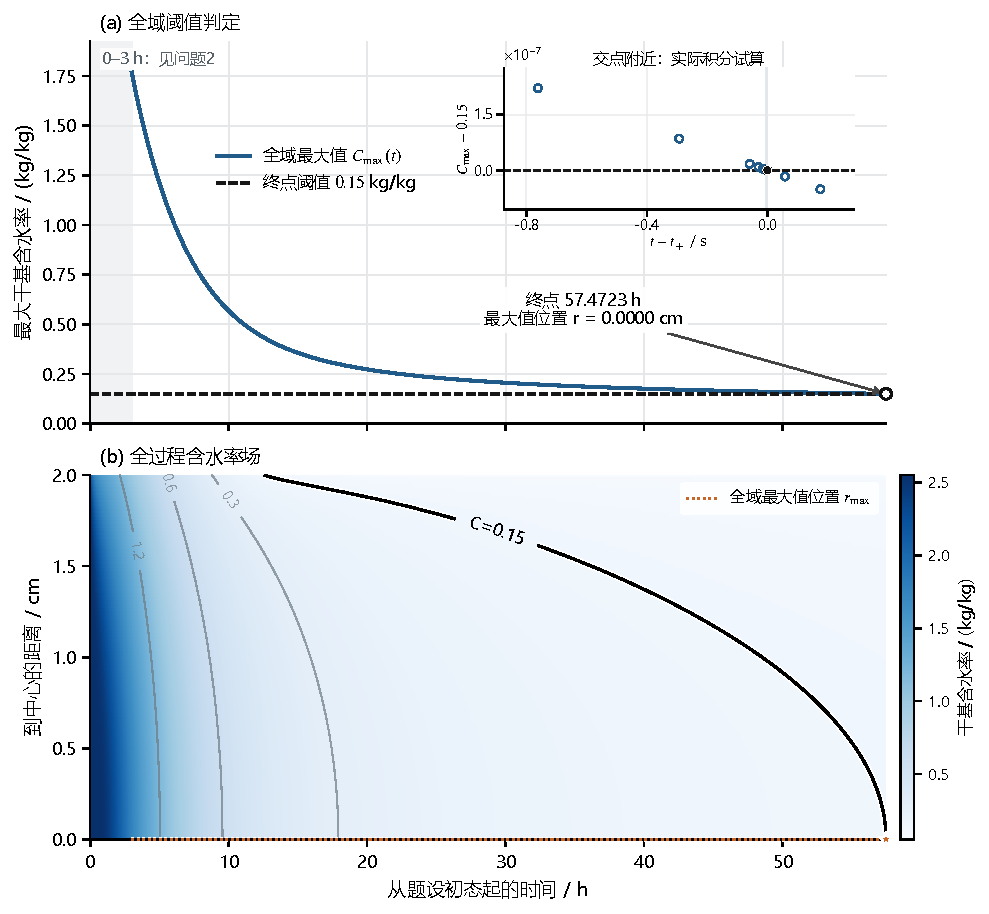
\includegraphics[width=0.96\linewidth]{q3/figures/fig5_q3_drying_endpoint.pdf}
\caption{全域最大含水率的阈值交叉及全过程含水率场。上幅从3 h的完整网格状态开始监测，
局部图为实际重新积分的事件试探点；下幅的0.15等值线展示各位置的达标顺序。}
\end{figure}

\subsection{数值验证与适用范围}
以不变的初始干物质质量为基准，定义
\begin{equation}
w_i=\frac{V_i}{\sum_jV_j},\qquad
B(t)=\sum_iw_iC_i(t)+L_2+L_3(t)-2.55.
\end{equation}
上述表达用于 $t\ge10800$ s，其中 $L_2$ 来自第二问完整前3 h的累计失水，$L_3$ 来自续算段表面通量，均以初始干物质质量归一化。
前3 h的残差使用第二问各时刻自身的累计失水计算，不将完整 $L_2$ 提前计入。
本次全过程最大绝对水量残差为 $2.540\times10^{-12}$ kg/kg。
续算步长由 $0.0625$ s 减至 $0.03125$ s，共同输出位置的最大含水率差为 $5.483\times10^{-7}$ kg/kg，达标时间差为 $0.09521484$ s。
空间对照固定续算步长 $\Delta t=0.25$ s、各网格第二问前缀的时间尺度 $\tau=\frac{1}{1024}$ s，原网格单元数由 $960$ 加至 $1280$，共同输出位置的最大含水率差为 $2.164\times10^{-6}$ kg/kg，达标时间差为 $0.04394531$ s。
空间对照固定续算步长 $\Delta t=0.25$ s、各网格第二问前缀的时间尺度 $\tau=\frac{1}{1024}$ s，原网格单元数由 $1280$ 加至 $1600$，共同输出位置的最大含水率差为 $1.002\times10^{-6}$ kg/kg，达标时间差为 $0.01464844$ s。
空间对照固定续算步长 $\Delta t=0.25$ s、各网格第二问前缀的时间尺度 $\tau=\frac{1}{1024}$ s，原网格单元数由 $960$ 加至 $1600$，共同输出位置的最大含水率差为 $3.165\times10^{-6}$ kg/kg，达标时间差为 $0.05859375$ s。
空间比较使用各网格各自的第二问完整末态，未进行网格投影。
事件夹逼、步长加密和网格加密分别核查；这些差值不是未知精确解的严格误差上界。
第二问前3 h只保留了采样场历史，因而最大值曲线从3 h开始，未用早期采样最大值冒充全域最大值。

在另一个匹配 $N=960,\Delta t=1$ s 的边界假设对照中，将4 h后的环境改为保持附件末值，得到总时长变化 $-18.1754$ min（$-0.5271\%$）。这体现输入延续假设的影响，不是离散误差或实验验证；正式结果仍采用事先确定的恒值延续。
模型沿用等效环境水分驱动、无显式潜热项及径向主导等假设，所得结果为模型预测。
数值收支、独立附录复现及输入延续对照不代替内部温湿场实验验证。
